
\begin{tabbox}{!t}

\caption{Survey response by gender, compared to total School staff count and gender distribution, and response rate by gender}
\label{tab:response:bygender}
\sisetup{
    group-digits=all,
    group-minimum-digits=4,
    group-separator = {,},
    table-format=4.1,
    mode=text,
    reset-text-series = false, 
    text-series-to-math = true,
    reset-text-family = false, 
    text-family-to-math = true
}
\footnotesize   
\begin{tabular}{p{4.5cm} 
                !{\qquad}
                S[table-format=2.0]
                !{\quad}
                S[table-format=2.1\%]
                p{0.5cm}
                S[table-format=2.0\%]                 
                !{\quad}
                S[table-format=2.1\%] 
                !{\qquad}
                S[table-format=2.1\%]                 
                } 

\toprule 
    & \multicolumn{2}{c}{\makecell{Gender representation\\of survey respondents}} 
    &
    & \multicolumn{2}{c}{\makecell{Gender representation\\of all staff School of CSIT}} 
    & {\multirow{2}{2cm}{\makecell{Overall\\Response\\rate}}}\\
    \cmidrule{2-3}\cmidrule{5-6}
Gender & {Count} & {\%} && {Count} & {\%} &  \\ 
\midrule 
Female & 16 & 28.6\% &&  19 & 23.5\% & 84.2\%\\
\hdashline
Male & 37 & 66.1\% && 62 &  76.5\% &59.7\%\\
\hdashline
Prefer not to say & 3 & 5.4\% && {n/a} & {n/a} & {n/a}\\
\midrule 
Total & 56 & 100.0\% && 81 & 100.0\% &69.1\%\\
\bottomrule 
\end{tabular}


\end{tabbox}


% \begin{SCfigure}[10][!ht]
% \hspace{-3pt}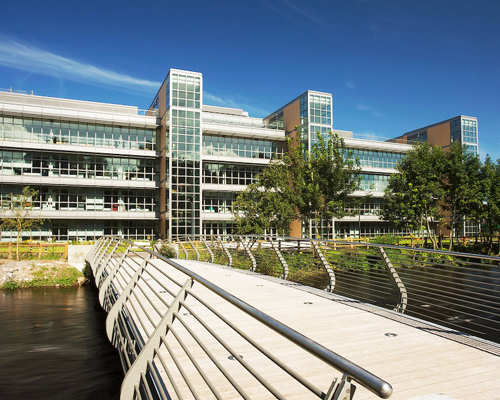
\includegraphics[width=3in]{img/WGB.jpg}
% \caption{Western Gateway Building: home to CSIT}
% \label{fig:wgb}
% \end{SCfigure}
